
\documentclass[12pt, a4paper, twoside, titlepage]{report}

%
% File containing all the package declarations
%
\usepackage{./tex/mystyle}

%----------------------------------------------------------------------------------------
%	DEFINITIONS
%----------------------------------------------------------------------------------------

\def \author {Katarzyna Sprawka}
\def \title {Numerical Assessment of Kidney Function from DCE-MRI}
\def \titlepl {Numeryczna ocena funkcjonowania nerek na podstawie obrazów DCE-MRI}
\def \supervisor {Prof. hab. dr inż. Andrzej Materka}
\def \auxiliarySupervisor {Dr inż. Marek Kociński}


%----------------------------------------------------------------------------------------
%	ABBRIVIATIONS
%----------------------------------------------------------------------------------------

\makeglossaries

\newacronym{ahrs}{AHRS}{\textbf{A}ttitude and \textbf{H}eading \textbf{R}eference \textbf{S}ystem} 
\newacronym{api}{\textbf{API}}{\textbf{A}pplication \textbf{P}rogramming \textbf{I}nterface}%
\newacronym{imu}{IMU}{ \textbf{I}nertial \textbf{M}easurements \textbf{U}nit}
\newacronym{json}{JSON} { \textbf{J}ava\textbf{S}cript \textbf{O}bject \textbf{N}otation}
\newacronym{vga}{VGA}{ \textbf{V}ideo \textbf{G}raphics \textbf{A}rray  ($640\times480$ px)}
\newacronym{wpf}{WPF}{ \textbf{W}indows \textbf{P}resentation \textbf{F}oundation}
\newacronym{xaml}{XAML}{ E\textbf{x}tended \textbf{A}pplication \textbf{M}arkup \textbf{L}anguage}


%----------------------------------------------------------------------------------------
%	BODY
%----------------------------------------------------------------------------------------


\begin{document}

% Abbriviations
% Abbriviations
\glsaddall
\printacronyms


% Title page
% Strona tytułowa

\thispagestyle{empty}

\begin{center}
	\vspace*{-1.5cm}
	{\scshape\LARGE Lodz University of Technology} \\ 
	{\scshape\large Faculty of Electrical, Electronic,\\Computer and Control Engineering } \\
	{\scshape\large Institute of Electronics} \\
	
	\vspace{2.0cm}
	{\scshape\large Master of Engineering Thesis } \\
	
	\vspace{0.5cm}
	\textbf{\Large\title{}} \\
	
	\vspace{0.5cm}
	\textbf{\Large\author{}} \\
	
	\vspace{1.5cm}
	\textbf{\large Student's number: 213407}
	\vspace{4.25cm}
	
	\begin{flushright}
		\em \rm {\large Supervisor:} \\
		\textbf{\large \supervisor{}} \\
		\em \rm {\large Auxiliary supervisor:} \\
		\textbf{\large \auxiliarySupervisor{}}
	\end{flushright}
	
	\vfill
	{\large Łódź, 2018}
\end{center}

% Po drugiej stronie strony tytułowej pusta strona
\newpage
\thispagestyle{empty}
\mbox{}

% Abstract 
%
% Streszczenie
%

\newpage	%░░░░░░░░░░░░░░░░░░░░▒▒▒▒▒▒▒▒▒▒▒▒▒▒▒▒▒▒▒▒░░░░░░░░░░░░░░░░░░░░
\thispagestyle{empty}
\pagenumbering{roman}
\setcounter{page}{1}

	\phantomsection \label{sec:Abstract}
	\addcontentsline{toc}{chapter}{Abstract}

	\begin{spacing}{1.0}
	\ifantyplagiat
	\else
		\begin{center}
			\vspace*{-3.35cm}
			{\scshape\normalsize Lodz University of Technology} \\ 
			{\scshape\normalsize Faculty Of Electrical, Electronic, Computer And Control Engineering} \\
			\vspace{1.15cm}	\textbf{\large\author{}} \\
			\vspace{0.3cm}
			{\scshape\footnotesize Master of Engineering Thesis} \\
			\vspace{0.25cm}
			\textbf{\large\title{}} \\
			\vspace{0.25cm}
			{Łódź, 2018~r.}
		\end{center}
		
		\begin{flushleft}
			{\supervisor{}}\\
			{\auxiliarySupervisor{}}\\
		\end{flushleft}
		\fi
		
		\begin{center}
			{\bf\large Abstract}
		\end{center}
	\end{spacing}
	
	\begin{spacing}{1.15}
		Tresc
	\end{spacing}
	
	
	
	
	\newpage
\thispagestyle{empty}
\mbox{}	%░░░░░░░░░░░░░░░░░░░░▒▒▒▒▒▒▒▒▒▒▒▒▒▒▒▒▒▒▒▒░░░░░░░░░░░░░░░░░░░░

	\newpage	
	\thispagestyle{empty}
	
	\phantomsection \label{sec:Streszczenie}
	\addcontentsline{toc}{chapter}{Streszczenie}
	
	\begin{spacing}{1.0}
	\ifantyplagiat
	\else
		\begin{center}
			\vspace*{-3.35cm}
			{\scshape\normalsize Technical University of Łódź} \\ 
			{\scshape\normalsize Wydział Elektrotechniki, Elektroniki, Informatyki i Automatyki} \\
			\vspace{1.15cm}	\textbf{\large\author{}} \\
			\vspace{0.3cm}
			{\scshape\footnotesize Praca dyplomowa magisterska} \\
			\vspace{0.25cm}
			\textbf{\large\titlepl{}} \\
			\vspace{0.25cm}
			{Łódź, 2012}
		\end{center}
		
		\begin{flushleft}
			{Supervisor: \supervisor{}}\\
			{Auxiliary supervisor: \auxiliarySupervisor{}}\\
		\end{flushleft}
		\fi
		
		\begin{center}
			{\bf\large Streszczenie}
		\end{center}
	\end{spacing}
	
	\begin{spacing}{1.15}
	tresc
	\end{spacing}
	
	
		\newpage
\thispagestyle{empty}
\mbox{}

	\newpage	%░░░░░░░░░░░░░░░░░░░░▒▒▒▒▒▒▒▒▒▒▒▒▒▒▒▒▒▒▒▒░░░░░░░░░░░░░░░░░░░░
	

% Acknowledgements
\chapter*{Acknowledgements}

\thispagestyle{empty}

\phantomsection \label{sec:acknowledgements}
	\addcontentsline{toc}{chapter}{Acknowledgementst}
	
First and foremost, I would like to express my sincere gratitude to Professor of the University of Bergen Arvid Lundervold for his enlightening guidance throughout this project and warm hosting me during the stay in Norway, for his encouragement and enthusiastic approach, immense knowledge, and most importantly for inspiring me with the world of medical imaging.

I also would like to thank my supervisors from my mother university, Professor Andrzej Materka and PhD.~Marek Kociński for the useful comments and remarks both the substantive and editorial ones, which helped to give this dissertation its final shape. Without their assistance this paper would have never been accomplished.

\newpage
\thispagestyle{empty}
\mbox{}	




% Content 
\phantomsection \label{sec:content}
\addcontentsline{toc}{chapter}{Contents}
	\begin{spacing}{1.1}
		\tableofcontents
	\end{spacing}
\newpage

%Introduction
\pagenumbering{arabic}
	\setcounter{page}{1}
	
\chapter*{Introduction}
	\addcontentsline{toc}{chapter}{Introduction}

\begin{comment}	
\lettrine[lines=3, slope=1em, findent=-0.8em]{A}{ccording to the beliefs of ancient Hebrews}, the kidneys were \cite{maio1999metaphorical}. Today, more mundane, but not less important functionality is being assigned to them. 

Kidneys, although often underestimated, are fundamental organs of human body and their working mechanism is extremely complex. Their essential task is to remove wastes from the organism but their functionality is much wider. They are also involved in maintaining acid-based balance, regulating the blood pressure and are major endocrine organs, which secret three important hormones: erythropoietin, calcitriol and renin. Besides the production, they also take part in degradation of hormones such as insulin or parathyroid hormon \cite{saladin}.

Gradually progressing loss of kidney function known as a chronic kidney desease is a~ growing world-wide problem. As much as 8--16\% of whole population suffers from this condition \cite{statistics}. It significantly decreases comfort of life and in extreme cases leads to death. What is more, it was shown that renal diseases are risk factor for development of cardiovascular diseases \cite{cardiovascular_diseases}.
Because of the fact that symptoms don't resemble renal failure, approximately 90\% of the ill are unconscious of it until late stages \cite{national_kidney_foundation}. That is way there is the demand for methods, which enable fast and accurate measurement of renal function required for all of three: prevention, monitoring and therapy.
The metrics of level of kidney function is glomelural filtration rate (GFR) \cite{traynor2006measure}. Not only does it allow for assessment how well our kidneys are working, but also it can determine the stage of kidney disease.
\end{comment}

% Chapter 1-Aims and scope of the project
\chapter{Aims and scope of the work}

To be done

% Chapter - The kidney
\chapter{The blood filter}
	
There is no life without metabolizing, and metabolism always produces variety of waste products, which accumulated in the tissues are toxic to the organism. Some of them are removed from the body by respiratory trucks, others through digestive system and some of them are extracted through the sweat gland. However, there is no doubt that the urinary system plays the major role in waste extraction.

The main organs of the urinary system are the kidneys. It is them, who perform the filtering function. The remaining ones,  ureters, urinary bladder, and urethra, form the urinary tracks and are responsible only for transforming and storing the urine. In this chapter the anatomy and physiology of the kidneys will be briefly introduced.

\section{Structure of the kidney} 

The kidneys are  bean-shaped, usually paired structures located at the back of the abdominal cavity in the retroperitoneal space. They lie on at the level of vertebrae T12 to L3.
The right kidney is slightly lower than the left one, because of the presence of the liver \cite{saladin, health_and_disease}. 

The average healthy adult kidney weights around 150\,g, is 11\,cm long, 6\,cm wide and 3\,cm thick \cite{kidney_dimensions, saladin}. As mentioned before, humans usually have two kidneys, however not always.  Some people are born with only one of them.  In such case, the present kidney is as heavy and big as the two kidneys together would be. In most cases it doesn't affect normal live. 

The kidneys are surrounded and protected by three types of connective tissue, from the outter part: 
\begin{inparaenum}[(1\upshape)]
\item \textit{renal fascia} anchoring the kidneys and the neighbouring organs to the abdominal wall
\item \textit{adipose capsule}, which is a layer of fat holding the kidney in a place
\item \textit{renal capsule}, made of fibrous tissue firmly enclosing the organ and protecting it from traumas and infections \cite{saladin, health_and_disease}.
\end{inparaenum} In the medial concave surface, there is a~slit called \textit{hillum}, which is the place where the  renal  artery enters and the renal vein and the ureter leave the kidney. The hillum extens into the \textit{renal sinus}, which is a large cavity occupied by blood and lymphatic vessels, nerves, urine-collecting structures and adipose tissue \cite{health_and_disease}.

The renal parenchyma is divided into two major parts: 
\begin{inparaenum}[(1\upshape)]
\item the outer 1\,cm thick portion of the kidney,  \textit{renal cortex}
\item the inner \textit{renal medulla}
 \cite{saladin, health_and_disease}.
\end{inparaenum}
The cortex projects into the kidney forming \textit{renal columns}, which divide the medulla into 10-14 \textit{renal pyramids}. Each of them has a characteristic shape of cone with wide base facing the cortex and the tip attached to the sinus called \textit{renal papilla}.  The papilla of the each pyramid points towards the \textit{minor calyx} collecting its urine. Few of them converge into the \textit{major calyx}, whereas the all latter ones form the funnel-shaped basin,  \textit{the renal pelvis}, which is the extension of the \textit{ureter} transforming the urine to the bladder \cite{saladin, health_and_disease, mosby}. The gross anatomy of the kidney is illustrated on the Figure \ref{fig:kidney_anatomy}.

	%\vspace*{-1.5cm}
\begin{figure}[H]
		\centering
		\includegraphics [height = 8cm]{kidney2}
		\caption [Gross kidney anatomy]{The structure of the kidney \cite{saladin}}
		\label{fig:kidney_anatomy}
	\end{figure}
\subsection{The nephron} 

As it is with most of the aspects of the human anatomy, the most interesting features of the kidney are invisible with naked-eye. 
The basic microscopic functional units of the kidney are nephrones. Above million of them enables the kidney to perform its functions \cite{health_and_disease}. Each of them is a tiny coiled tube, the \textit{renal tubule}, with a bulb at the end, the \textit{renal corpuscle}, and extends through both the cortex and the medulla. 

The renal corpuscle is composed of the two-layered \textit{glomerular (Bowman) capsule} enclosing the
\textit{glomelurus}, which is a cluster of capillaries. The renal tubule is a~duct leading from the glomelural capsule to the pyramid papilla. It can be divided into several regions, subsequently from the glomerular corpuscle: 
\begin{inparaenum}[(1\upshape)]
\item The \textit{proximal convoluted tubule} (PCT)
\item the \textit{nephron loop (loop of Henle)}, which consists of the \textit{descending and ascending limbs}
\item The \textit{distal convoluted tubule }(DCT)
\item the \textit{collecting duct} receiving the fluids from the DCTs of few nephrons. Multiple of them merge and form papillary ducts, which lead  to the minor calyx.
% \cite{saladin, health_and_disease}.
\end{inparaenum}
Each of the segment has individual cellular appearance and function.

Every functional unit of the kidney is supplied with the blood by the small blood vessel called \textit{the proximal convoluted tubule} whereas the \textit{efferent  arteriole} takes it back. The blood leaving the nephron, flows  into  a
network of \textit{peritubular  capillaries} surrounding the renal tubule. The particular parts of the nephron are depicted on the Figure \ref{fig:nephron}.

\begin{figure}
		\centering
		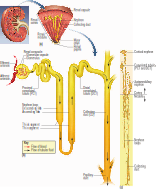
\includegraphics [width = \textwidth]{nephron}
		\caption [nephron]{The structure of the kidney \cite{saladin}}
		\label{fig:nephron}
	\end{figure}



\section{Functions of the kidney} 

Despite of the fact that the key function of the kidneys is purifying the blood, the other ones are equally important. Kidneys are responsible for maintaining homeostasis of all body due to which, all organs can work in optimal environment.
It is crucial for proper functioning of whole organism \cite{mosby}. One can conclude that the role of kidneys is enormously important. The kidneys are involved in the following processes:
\begin{description}
		%\renewcommand\labelitemi{$\blacksquare$}
		\item [Blood filtering.] The kidneys filter the blood from metabolic waste, excess salt and toxins and then excrete unwanted substances in the urine \cite{saladin, health_and_disease, mosby}.
		
		\item [Osmoregulation.]	For proper functioning of the organism, the concentration of the salts in the body has to remain relatively the same. The kidneys, influence this concentration which by controlling the amount of water and solutes excrected from the organism \cite{sturkie1986kidneys}.	
		
		\item [Maintainance of water balance.] The kidneys controll the amount of water conserved and eliminated in the urine so that the amount of body water remains on the stable level \cite{jequier2010water}.
					
		\item [Blood pressure regulation.] Maintaining appropriate blood pressure is achieved in 2 ways: \begin{inparaenum}[(1\upshape)]\item if the blood pressure drops, the kidneys release the enzyme \textit{renin}, which activates a blood protein \textit{angiotensin} making the blood vessels to constrict. What is more, angiotensin triggers the mechanism which increases the absorption of water and sodium increasing blood volume  \item regulating the amount of water, which was mentioned before \cite{guyton1972arterial}. \end{inparaenum} 
			
		\item [Maintainance of the acid-base balance.] The food conteained in our diet can acidify or neutralize the organism. If the pH is outside the tolereable boundaries, enzymes and proteins break down, which in extreme cases can lead to death. Kidneys in collaboration with the lungs are responsible for maintaining healthy pH of the body fluids. While the lungs' task is to regulate carbon dioxide ($CO_{2}$) concentration, the kidney acts by reabsorbing or regenerating bicarbonate ($HCO_{3}^{-}$) from urine and excreting hydrogen ions and fixed acids into it \cite{hamm2015acid}.
	
	\item [Red blood cell production.] If the level of oxygen in the tissue is insufficient, the kidneys release \textit{erythroprotein}, the hormon stimulating the bone narrow to red blood cells production \cite{donnelly2001erythropoietin}. 

\item [Keeping the bones strong.] The kidneys, together with the liver, synthesize the active form of vitamin D called \textit{calcitriol} (1,25-dihydroxycholecalciferol) enabling the body to absorb calcium and phosphorus, crucial minerals for strengthening the bones \cite{williams2009vitamin}.

\item [Prevent the hunger.] In the situation of extreme starvation, the kidneys can synthesize glucose from non-carbohydrate carbon substrates breakind down the other molecules. This phenomena is known as \textit{gluconeogenesis} \cite{newsholme1967control}.

\item [Hormones degradation.] The kidneys takes part in degradation of hormones such as \textit{parathyroid hormone} or \textit{insulin} \cite{emmanouel1980role}. 
%					
	\end{description} 

\subsection{Urine formation} 
Everyday, our kidney filter as much as 200 litres of fluid and excrete 1.5 litres of urine. The process of the urine formation can be divided into 3 stages:
\begin{enumerate}
\item{\textbf{Glomerular filtration}} When the blood enters the glomerulus through the afferent arteriole, the first step begins.  
\item{\textbf{Tubular reabsorption}}
\item{\textbf{Tubular secretion}}
\end{enumerate}


\subsection{glomerular filtration rate}

\section{Kidney diseases} 

 

% Chapter - DCE-MRI
\chapter{Dynamic contrast enhanced MRI}
	
Medical Imaging started with the development of X-rays by Wilhelm Röntgen in 1895, for which he received a Nobel Price \cite{rontgen1896new}. 
An enormous progress has been done since that time and numerous different imaging methods were developed, which found various applications in the medical field. Possibility of creating the visual representations of human interior as well as the processes occurring in tissues and organs, and thus their functionality, much facilitated medical diagnosis and prognosis.   
Some imaging techniques have became an integral part of clinical care (i.e computer tomography, magnetic resonance imaging, positron emission tomography), whereas there exist one, which still needs to prove its utility. 

In this chapter the imaging technique, which is DCE-MRI will be introduced and its mechanism of imaging will be presented.

\section{Fundamentals of MRI}
In order to understand the mechanism of acquiring DCE-MRI sequences, it is inevitable to introduce the principle of operation of \textit{Magnetic Resonance Imaging}~(MRI).

MRI is an imaging technique based on the phenomena of induced nuclear  magnetism in the patient. Every molecule possessing a nuclei with an odd number of protons or neutrons  have a spin, implying a weak though observable randomly oriented nuclear magnetic moment. 
This particles include for example \textsuperscript{1}H, \textsuperscript{13}C, \textsuperscript{31}P, \textsuperscript{23}Na, \textsuperscript{19}F \nocite{bronzino1999biomedical}\cite{biomedical_hanbook_imaging, grover2015magnetic}. If placed in a strong static magnetic field, these moments strongly tend to align parallel to the external field. Some of them will align antiparallel to the field, however there will always be an excess of these directed towards the direction of the field, as this state is more energetically stable. The resulting net magnetic moment, $M_0$, will be directed with the external field \cite{bushong2014magnetic}.

Magnetic resonance imaging explicit the fact that the human body in 80\% consists of water. During the MRI examination, the object is placed in the scanner producing strong magnetic field, which causes the hydrogen atoms to align in the direction of the field, pointing towards the head of the object as shown in Figure~\ref{fig:magnetic_field} \cite{bushong2014magnetic}. 

\begin{figure}
		\centering
		\includegraphics [width =13cm]{magnetic_field}
		\caption [Hydrogen atoms placed in the magnetic field]{Hydrogen atoms located in a human body placed in the strong magnetic field ($B_{0}$), generated by the MRI scanner, align to the direction of that field \cite{magnes}}
		\label{fig:magnetic_field}
	\end{figure}

In addition, atoms have an angular momentum making them precess about the magnetic field direction with a frequency $\omega_{0}$, called the \textit{Larmor frequency}, which is proportional to the field:   
\begin{equation}
\omega_{0} = \gamma{}B_{0}\:,
\label{eq:larmor}
\end{equation}
where $\gamma$ is the nuclei specific constant \textit{gyromagnetic ratio} (for hydrogen equal to 42.6\,MHz/T) and $B_{0}$ is the strength of the external magnetic field \cite{biomedical_hanbook_imaging, bushong2014magnetic}. This preccessional motion is is shown in Figure~\ref{fig:larmor}.

\begin{figure}
		\captionsetup{aboveskip = 10pt}
		\centering
		\includegraphics [width =5cm]{larmor}
		\caption [Precessional motion of the atom in the magnetic field]{Hydrogen atom placed in a strong magnetic field $B_0$ precesses about the direction of that field with the frequency $\omega_{0}$}
		\label{fig:larmor}
	\end{figure}
Further, when the radio-frequency (RF) pulse equal to the Larmor frequency is applied perpendicularly to the magnetic field, the resonance occurs. The atoms absorb the energy, transits to the higher energy state and flip to the other position.
When the RF transmission is stopped, the atoms return to their equilibrium state (realign to the field $B_{0})$ releasing the energy as a radiation signal, referred to as \textit{free-induction decay} (FID) response signal, which is picked by MRI receiver. This return to equilibrium is called \textit{relaxation}. The relaxation time as well as the amount of the energy released strongly depends on the magnetic properties of the tissue, which means that every tissue generates different response signal. The dedicated software analyses and processes obtained signal, which is a combination of numerous response signals from all excited atoms and generates the~image \cite{biomedical_hanbook_imaging, bushong2014magnetic}.    

During the MRI examination, the strength of the magnetic field produced by the scanner varies along the body, so that the Larmor frequency is different for different regions. By changing frequency of emitted RF, the appropriate part can be imagined. 

The typical MRI scanner consists of:
\begin{enumerate}
\item \textbf{The main field magnets}, which produces strong, uniform magnetic field polarizing the sample \cite{biomedical_hanbook_imaging}. Typical strength of the field of a clinical MRI scanner ranges between 0.2--1.5\,T, whereas research systems reaches values even up to 21\,T for animal models \cite{grover2015magnetic, sharma200821}.
\item \textbf{Shim coils.} In clinical practice, the main field magnets never produce perfectly uniform field so the shim coils adjusting its homogeneity have to be used \cite{biomedical_hanbook_imaging}.
\item \textbf{Gradient coils} producing three secondary gradient magnetic fields in each of the \textit{x-}, \textit{y-} and \textit{z-} direction. In this way, the resonance frequency of protons varies as a function of position, which enables encoding the spatial position and imaging of thin anatomic slices \cite{hidalgo2010theory}.
\item \textbf{RF system}, task of which is to excite the hydrogen atoms and to receive their FID response signal \cite{biomedical_hanbook_imaging}
\item \textbf{The processing unit of high performance} controlling the system and processing the received combination of response signals \cite{biomedical_hanbook_imaging}.
\end{enumerate}

\subsection{\textit{T\textsubscript{1}-} and \textit{T\textsubscript{2}-}weighted images}

Although, there are few approaches of obtaining the contrast between different tissues in an image, utilizing different tissue properties, most widely used in clinical applications are these based on the relaxation of the magnetization. However, there are two kinds of relaxation, and thus two mechanisms of creating the MRI image can be distinguished \cite{biomedical_hanbook_imaging}.
\begin{description}
		\item [\textit{T\textsubscript{1}-}weighted images] exploits spin–lattice relaxation, characterised by the time \textit{T\textsubscript{1}}, which describes the time required by excited atoms to return to the equilibrium state after it was altered by the RF pulse. This mechanism is shown in Figure \ref{fig:t1plot}. Sometimes the acquiring of \textit{T\textsubscript{1}}-weighted sequence is preceded by the injection of \textit{gadolinium}, paramagnetic contrast agent (CA), which  shortens time \textit{T\textsubscript{1}} and appears very bright on the image. This property is especially useful while visualising vascular structures or brain tumours and abscesses blocking a blood supply \cite{biomedical_hanbook_imaging, grover2015magnetic}.   
		
		\item [\textit{T\textsubscript{2}-}weighted images] are based on spin-to-spin relaxation, described by the \textit{T\textsubscript{2}} indicating the time required by the nuclei response signal to decay after it has been created \cite{biomedical_hanbook_imaging, grover2015magnetic}. \textit{T\textsubscript{2}} contrast is presented in Figure~\ref{fig:t2plot}. 
\end{description}
\begin{figure}[H]
\captionsetup[subfloat]{captionskip=0.5cm}
	\centering
	\subfloat[\textit{T\textsubscript{1}} contrast]{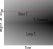
\includegraphics[height=6.25 cm]{t1plot}\label{fig:t1plot}}\hspace{1.5cm}
	\subfloat[\textit{T\textsubscript{2}} contrast]{\includegraphics[height=6.25 cm]{t2plot}\label{fig:t2plot}}\\	
\vspace{0.5cm}
\caption[\textit{T\textsubscript{1}} and \textit{T\textsubscript{2}} contrast mechanisms]{\textit{T\textsubscript{1}} and \textit{T\textsubscript{2}} contrast mechanisms \cite{biomedical_hanbook_imaging}}
\label{fig:t1t2plot}
\end{figure}

Examples of the images acquired using described above two basic mechanisms are shown in Figure \ref{fig:t1t2}a-b. 
The figure presents identical axial section of a healthy person's brain. In the \textit{T\textsubscript{1}} weighted  image, one can notice ring of subcutaneous fat, which is bright due to its short spin–lattice relaxation time. Gray matter has longer \textit{T\textsubscript{1}} than white matter, so it appears darker. In the second picture, utilizing the \textit{T\textsubscript{2}} difference between tissues, cerebrospinal fluid in the ventricles appears very bright due to its long  \textit{T\textsubscript{2}}. \textit{T\textsubscript{2}} of the white matter is shorter that those of gray matter, which makes the latter one brighter. \textit{T\textsubscript{1}} and \textit{T\textsubscript{2}} weighted images are only two of the few contrast mechanisms used in  MRI and the choice of appropriate one strongly depends on the application and the region of interest under examination \cite{biomedical_hanbook_imaging}.

 
\begin{figure}

\captionsetup[subfloat]{captionskip=0.5cm}
	\centering
	\subfloat[\textit{T1}-weighted image of a brain]{\includegraphics[height=6.5 cm]{t1}}\hspace{1.5cm}
	\subfloat[\textit{T2}-weighted image of a brain]{\includegraphics[height=6.5 cm]{t2}}\\	
\vspace{0.5cm}
\caption[Comparison of \textit{T\textsubscript{1}}- and \textit{T\textsubscript{2}}-weighted images]{Example MRI image of a brain of a healthy volunteer demonstrating T1 and T2 contrast \cite{t1t2brain}}
\label{fig:t1t2}
\end{figure}

Currently MRI is one of the most widely used medical imaging techniques applied to the all parts of a body. It allows to create the detailed anatomical images in axial, sagittal, coronal or even oblique plane. During the MRI examination subsequent thin 2D \textit{slices} along chosen axis are produced, which makes it a tomographic imaging method. As a result, during imaging sequence, a large dataset is acquired, from which any anatomical section can be reconstructed or a 3D model of a region of interest can be assembled \cite {bushong2014magnetic}. Another advantage of MRI is not using any harmful ionizing radiation.

The clicical applications of MRI include diagnosis of blood vessel damages, multiple sclerosis, brain injuries, spinal cord injuries, brain strokes, blocked blood vessels, heart diseases, damages caused by a heart attack, bone infections, differnet kind of tumors and cancers and many more \cite{mriApplications}.

\vspace{15pt}
\section{DCE-MRI}
\textit{Dynamic contrast enhanced magnetic resonance imaging} boils down to the acquisition of multiple MRI scans, with addition of one signifcant component---the time domain \cite{jackson2005dynamic}. 
During the examination a contrast agent is injected in the peripheral vein into the bloodstream and the \textit{T1}-weighted images are acquired with fast imaging technique. 
The passage of the tracer through the target tissue results in changes in signal intensities over the time.
The kinetics of the CA, so its temporal and spatial distribution is strongly dependent on the physiological parameters such as tissue perfusion, volume of the extravascular and extracellular space and vessel permeability, and thus the analysis of so obtained intensity changes as a~function of time, $S(t)$, provides important functional information \cite{bokacheva2008assessment, khalifa2014models}. 
As an example, malignant tumours show faster and higher levels of enhancement 
than normally functioning tissue, which is associated with tumour's increased vascularity and higher endothelial permeability to the CA \cite{jackson2005dynamic}.


\newpage
\subsection{DCE-MRI analysis}
There are many methods of time-courses analysis obtained during DCE-MRI. In general, they can be divided into qualitative, semi-quantitative and quantitative ones \cite{barnes2012practical}.
All methods can be applied voxel-wise or to the whole Region of Interest~(ROI), where the average time-intensity curve is produced from the voxels values within the ROI \cite{khalifa2014models}. 

\subsubsection{Qualitative analysis}
In traditional approach, the evaluation of the time-intensity curves is performed by experienced observer via subjective visual inspection, who's task is to classify the curve to one of the three predefined enhancement patterns. This three templates are shown in Figure~\ref{fig:patterns}. 

\begin{figure}[h!]
		\centering
		\includegraphics [width =8cm]{dcemri_patterns}
		\caption [DCE-MRI enhacement patterns]{Different DCE-MRI enhacement patterns \cite{khalifa2014models}}
		\label{fig:patterns}
	\end{figure}

Type~I defines a shape characterized by the gradual increase of the signal intensity during the whole acquisition time. In type~II, after the initial peak, the plateau occurs---the curve remains relatively constant. Type~III is associated with the decrease in signal intensity after the peak signal intensity \cite{barnes2012practical}.
In this way, i.e the tumour can be distinguished from the healthy tissue.

Although the qualitative analysis is a very convenient one as it does not require any additional data and calculation, its  major disadvantage is not delivering any quantitative parameters and being fully dependent on the observer's experience. \vspace{10pt}

\subsubsection{Semi-quantitative analysis}
The semi-quantitative analysis incorporates calculation of parameters directly from the time-intensity curve characterizing its shape \cite{khalifa2014models, barnes2012practical}. Several examples of the parameters include \textit{onset time} ($T_o$), \textit{maximum signal intensity} ($S_m$), \textit{peak enhancement} ($\Delta S$), \textit{time to peak} ($T_p$), \textit{wash-in slope}, \textit{wash out slope}, \textit{average plateau},  \textit{area under the curve} (AUC) or \textit{initial uptake area under the curve} (IAUC) \cite{khalifa2014models}. Listed parameters are depicted in Figure~\ref{fig:parameters}. 

\begin{figure}[h!]
		\captionsetup{aboveskip = 12pt}
		\centering
		\includegraphics [width =10.5cm]{semi}
		\caption [Sample paramterers used in semi-quantitative DCE-MRI analysis]{An example of the time-intensity curve, $S(t)$, with depicted metrics explored  in semi-quantitative DCE-MRI analysis. Note that $S_0$ is the signal intensity before CA arrival whereas $S_{final}$ is the intensity registered in the last temporal point at the end of the experiment $T_{max}$ \cite{khalifa2014models}}
		\label{fig:parameters}
	\end{figure}

As in the case of previous method, the ease of the calculations performed directly from the curve is its biggest advantage.  However obtained empirical parameters in some way correlate with tissue physiology, i.e. increased vascular density
or permeability usually increases the wash-in slope, AUC, and peak enhancement,
in the same time decreasing the time to peak, it is difficult to relate them directly to some particular physiological quantities \cite{barnes2012practical}.

\subsubsection{Quantitative analysis}
Quantitative assessment of the $S(t)$ curve is surely the most sophisticated one.
It involves fitting one of the several quantitative  mathematical  models, which  describes  the pharmacokinetics  of  the  contrast  agent to the concentration-time curve of the target tissue.
Not only does this type of analysis require acquisition of the intensity-time curve of the feeding blood vessel next to that of the target tissue but also one has to convert obtained curves into CA concentration-time curves. In reward, some physiologically interpretable kinetic parameters of the tissue are estimated \cite{jackson2005dynamic, barnes2012practical}. 
The issue of the pharmacokinetic modelling in details is described in Chapter~{\ref{chapter:pk}.

\subsection{DCE-MRI applications}
Even though not present in clinical routine yet, over the last two decades DCE-MRI has been widely explored in clinical studies.
There is no doubt that obtaining important functional information next to the anatomical one in a single imaging session is one of the biggest advantage of Dynamic Contrast Enhanced MRI. It has shown to have great potential in early detection of breast cancer, providing higher sensitivity than classical mammography, as well as detection of small lesions, which classical MRI is not capable to. What is more, it showed promising results in accurate localisation of prostate cancer. Further DCE-MRI was found to be reliable technique of monitoring tumour responses for treatment (changes in vascular support). DCE-MRI also showed its effectiveness in accurate detection of renal rejection.
Last but not least, what is of great importance for this project, from the DCE-MRI images, important physiological parameters of the tissue, such as GFR of the kidney can be estimated   \cite{khalifa2014models}.

The mentioned findings, which are only a drop in the ocean of researches,  suggest that DCE-MRI is a relevant non-invasive imaging technique, which can be a~part of clinical care used in a really wide range of applications. 

% Chapter - Principles of pharmacokinetic modelling
\chapter{Pharmacokinetic modelling}
\label{chapter:pk}

The ideal output obtained from DCE-MRI analysis would be some reliable quantitative physiological parameters of the tissue under examination. Numerical results, however, always call for some mathematical description of the system under examination. 

The time-dependent distribution and deposition of a substance in a living system can be described by Phamacokinetic (PK) models~\cite{gerlowski1983physiologically}. First attempts of depicting the organism by a set of components were performed by Torsten Teorell in 1937. He then created a model of whole body shown in Figure \ref{fig:pk_draft} and described the processes inside by a set of differential equations in the same time presenting  their solutions~\cite{pkfather}. Teorell is now considered  a father of \textit{Pharmacokinetic} (PK) modelling. 

\begin{figure}[t]
		\centering
		\includegraphics[height =11cm]{pk_draft}
		\caption [Teorell's first PK model]{First PK model desribed by Teorell \cite{pkfather}}
		\label{fig:pk_draft}
	\end{figure}

PK models aim to characterise a physiologic system, not necessarily the whole body, by decomposing it into interacting compartments. Every of them is a homogenous, well-mixed space with the uniform tracer distribution \cite{PMID:20540902}.
Thus, the multicompartment system reaches the equilibrum in different time.  PK models have very wide clinical application: from estimating the optimal drug dose to determining safe working environment while working with toxins  \cite{gerlowski1983physiologically}.

Given the fact that the contrast agent used in DCE-MRI examination can be considered as a substance flowing through the organism, Pharmacokintetic modelling can also be used in analysis of so obtained data.   
This approach, called the quantitative one, is based on fitting mathematical model to acquired tissue concentration time courses \cite{khalifa2014models, jackson2005dynamic, barnes2012practical}. In this way, the quantitative parameters can be assessed, which cannot be overestimated while evaluating the tissue function. 


This chapter deals with the approach of PK modelling giving the brief inside in its basic principles and requirements with focus on DCE-MRI applications. 
\newpage



\section{The tracer kinetic theory} 
The compartment PK models describe complex blood-tissue exchanges. The general tracer kinetic theory is based on  principle of mass conservation and PK models are formulated as mass balance equations \cite{khalifa2014models, thesis}. 
\begin{figure}[H]
\captionsetup[subfloat]{captionskip=0.5cm}
	\centering
	\subfloat [An arbitrary tissue]{\includegraphics[width=0.5\linewidth]{model1}\label{fig:model1}}
	\subfloat[An arbitrary multi-compartment model]{\includegraphics[width=0.5\linewidth]{model2}\label{fig:model2}}\\	
\vspace{0.5cm}
\caption[An arbitrary multi-compartment model]{An arbitrary tissue with a possible compartmental architecture. The system (square) has one inlet and one outlet.
The tracer in the volume of distribution is
indicated in dark green in (a). $J_{12}$ and $J_{21}$ are fluxes between compartments (oval shaped)}
\label{fig:model}
\end{figure}
\noindent Given the tissue with at least one inlet and one outlet (see Figure~\ref{fig:model}a), the time-varying tracer concentration in the tissue, $C_t(t)$ can be expressed as \cite{thesis}:
\begin{equation}
C_t(t) = \frac{M_t(t)}{V_t},
\label{eq:pk1}
\end{equation}
where $M_t(t)$ is the amount of tracer in the tissue (in mmol) and $V_t$ is the volume of the tissue (mL). The \textit{flux} (mmol/mL/min) in terms, is the amount of the tracer, which travels through an inlet or outlet per unit time. After the normalisation to the unit tissue volume the flux can be expressed as \cite{thesis}:
\begin{equation}
J(t) = \frac{1}{V_t}\frac{\partial M_t(t)}{\partial t}
\label{eq:pk2}
\end{equation} 
Let's now consider an arbitrary multi-compartment model composed of $n$ interacting compartments. Then, the outlet of one compartment is in the same time the inlet of another, see Figure~\ref{fig:model}b. The tissue concentration in such a system is defined as \cite{thesis}:   
\begin{equation}
C_t(t) = \sum_{j=1}^{n}v_jC_j(t),
\label{eq:pk3}
\end{equation}
where $v_j\leq1$ is the \textit{fractional volume} (dimensionless) of $j$th compartment and $C_j$ is the concentration of tracer in this compartment. 
From the principle of the conservation of the mass it is known that no amount of the indicator is neither created nor destroyed in the tissue. Under such condition, applying the mass balance equation to the every of the compartments, the change of the total amount of substance in the compartment is given by \cite{thesis}:
\begin{equation}
\frac{dM_j(t)}{dt} = \sum_{i=1}^{I}\frac{M_i(t)}{\partial t}-\sum_{o=1}^{O}\frac{M_o(t)}{\partial t} ,
\label{eq:pk4}
\end{equation}
where $I$ and $O$ are the number of inlets and outlets of the compartment respectively. 
After normalisation to the unit tissue volume \cite{thesis}:
\begin{equation}
vj\frac{dC_j(t)}{dt} = \sum_{i=1}^{I}J_i(t)-\sum_{o=1}^{O}J_o(t) ,
\label{eq:pk5}
\end{equation}
The mass conservation principle implies that the amount of the substance transported from a compartment $i$ to a compartment $j$ per unit time is equal to the amount of the given substance leaving the $i$. This leads to the formula \cite{thesis}:
\begin{equation}
\frac{\partial M_{ij}(t)}{\partial t} = k_{ep}M_i,
\label{eq:pk6}
\end{equation}
where $k_{ep}$ is so called \textit{rate constant} (in min$^{-1}$). Again, after the normalisation to the unit tissue volume \cite{thesis}:
\begin{equation}
J_{ij}(t) = K_{trans}C_i(t),
\label{eq:pk7}
\end{equation}
where $K_{trans}=k_{ep}v_j$ is \textit{transfer constant} (in ml$^{-1}$). $K_{trans}$ combines both the flow and tissue permeability. Some approaches allow their separate estimation by differentiating the \textit{flow} $F$ by the \textit{permeability surface area product}, $PS$ \cite{thesis}. 

\subsection{Linear stationary systems}
All PK models are based on two fundamental assumptions, without which solving the models' equations would not be possible: that the system is linear and stationary. Hence the response of the influx is proportional to the dose of the injected tracer \cite{thesis, sourbron2011scope} 

For any linear and stationary system satisfying the 
initial condition $C_t(0) = 0$, which means $t = 0$ is chosen before tracer injection,
the tissue concentration can be obtained by convolving the concentration of tracer input function with the Impulse Response Function (IRF) of the tissue denotated as $h(t)$ \cite{sourbron2011scope}: 
\begin{equation}
	\label{eq:convolution}
	C_{t}(t) = C_{in}(t)\circledast h(t) = \int_{0}^{t}C_{in}(\tau)h(t-\tau)d\tau 
\end{equation}
When the only inlet of the examined tissue is an artery, the input function corresponds to the function of plasma concentration at the entrance of the system and can be derived from so-called \textit{Arterial Input Function} (AIF), $C_{in} = C_{p}$. The IRF in terms can be found by applying the Laplace transform to the appropriate mass balance equations \cite{thesis}.
\newpage

\subsection{One-compartment model}
For better understanding, the above theory will be explained on an example one-compartment model, but the reasoning is similar to the all models used in this work. Given a~one-compartment system with a single inlet and outlet and taking into consideration that all substances in the system have constant volume, it is known that inflow have to level the outflow. On the basis of Formulas \ref{eq:pk5}, \ref{eq:pk7} the mass balance equation of the system can be formulated as follows \cite{thesis}:
\begin{equation}
v_1\frac{dC_1(t)}{dt} = K_{trans}(C_{in}(t)-C_1(t)),
\end{equation}
where the $v_1$ is the fractional volume of the compartment. From the Formula \ref{eq:pk3} \cite{thesis}:
\begin{equation}
\frac{dC_t(t)}{dt} = K_{trans}(C_{in}(t)-C_t(t)/v_1),
\label{eq:laplace}
\end{equation}
Assuming that $C_{in}$ is a short pulse of concentration, $C_{in}=\delta(t)$ the IRF of the tissue can be obtained by applying the Laplace transform to the Formula \ref{eq:laplace}: 

\begin{equation}
\mathcal{L}\{\dot{h}\}(s) = K_{trans}(\mathcal{L}\{\delta\}(s)) - \frac{K_{trans}}{v_1}(\mathcal{L}\{h\}(s))
\end{equation}
The solution is \cite{thesis}:
\begin{equation}
h(t) = K_{trans}e^{-k_{ep}t}
\end{equation}
Finally, according to the Formula~\ref{eq:convolution}, the tracer concentration in the tissue can be expressed as \cite{thesis}:
\begin{equation}
	C_{t}(t) = C_{in}(t)\circledast  K_{trans}e^{-k_{ep}t} 
\end{equation}


The described above physical and mathematical background was shortened so that to indroduce very basics and explain enough but not too much on the theory of PK models. If the reader is interested, I kindly refer to the original sources \cite{sourbron2011scope, thesis}. 

There exist numerous PK compartment models used in DCE-MRI analysis and every of them is based on different assumptions and simplifications, which are not proper in all cases. The choice of the model depends on such factors as a type of a~tissue under concideration, the quality of data, the possibility of obtaining AIF and many more \cite{khalifa2014models}. One should, however, remember that no mathematical equations will ever describe the living organism accurately in 100\% as there are no two samples of tissue behaving exactly in the same way. The most widely used PK models include: \textit{Toft and Keromode} (TK), \textit{Extended TK} (ETK), \textit{Two-compartment Exchange} (2CXM) and \textit{Patlak} (PM) models.  

\section{Arterial Input Function}
The quantitative approaches of DCE-MRI analysis require obtaining the input function delivering the tracer to the system. From the physiological point of view, the tracer is delivered to the tissue of interest through the feeding blood vessels, so the input function becomes the plasma concentration, $C_p$ in these vessels. Plasma concentration can be obtained from so-called \textit{Arterial Input Function} (AIF), which describes the changes of the tracer concentration in the feeding blood source. Its tracer kinetics differs significantly from this of the tissue. The changes in plasma concentration are fast and sharp and it is of great importance to cover the rapid peak of the signal or else the important information about the tissue will be lost \cite{khalifa2014models, jackson2005dynamic, barnes2012practical}.   
In general there are three approaches of acquiring the AIF:
\begin{enumerate}
\item{\textbf{Gold standard AIF}} is obtained by blood sampling during DCE-MRI examination.
Although its accuracy strongly depends on the frequency of collected samples, this method usually allows accurate measurement of the AIF, but is inconvenient for both the patient and the examiner.
What is more, in some cases, for example during DCE-MRI of a breast, blood collection close to the tissue of interest is impossible to perform due to the lack of big vessels in this region \cite{khalifa2014models, barnes2012practical}. 
\item{\textbf{DCE-MRI AIF}} is determined directly from the obtained DCE-MRI data. In this approach the time-varying signal intensity from the region containing large feeding artery is converted into the tracer concentration in this way estimating the AIF. The major limitation is that it is not always possible to cover the the desired artery in the DCE-MRI acquisition field, for example during imaging small lesions in a breast \cite{khalifa2014models}.   
\item{\textbf{Population-based AIF}} is obtained by averaging the AIF of the group of subjects to be used in subsequent studies of the similar subjects. Because the need of acquiring subject-specific AIF is eliminated, the temporal resolution of the DCE-MRI can be decreased (CA tissue kinetics is slower than in the blood) in the same time increasing the quality of the images or the spatial resolution. The biggest disadvantage of this method is possible variance between individual AIFs \cite{jackson2005dynamic}. 
\end{enumerate}



\section{Intensity to concentration conversion}
Because the PK models describe kinetics of the system in terms of the CA concentration in the tissue and the output of DCE-MRI examination is the signal intensity as a~function of time, the conversion of the signal intensity to concentration is indispensable. 
As long as the relationship between CA concentration and the signal intensity  is linear, and the same for both the tissue and the blood in case of acquiring AIF from DCE-MRI images, the conversion boils down to the substarcting the baseline so that the concentration before the tracer arrival is at the level of 0. This conditions are satisfied at low doses of CA \cite{khalifa2014models}.

At high doses of the CA, however, this linearity is not true anymore due to the saturation effect of the signal. Non-linearity adds one more complication to the DCE-MRI examination. In such case, in order to convert the signal intensity into the CA concentration, the maps of the native relaxation time, $T_{10}$, which is the value of $T_1$ before the tracer injection, have to be measured. Then, the values can be substituted to the Formulas \ref{eq:conversion2}, \ref{eq:conversion3} and the CA concentration can be obtained \cite{khalifa2014models, jackson2005dynamic, barnes2012practical}.


The dependency between the CA concentration in the tissue, $C_t(t)$  and the relaxation rate, $1/T_1(t)$ is given by the Solomon-Bloembergen equation \cite{jackson2005dynamic}:
 \begin{equation}
 \frac{1}{T_1(t)} = \frac{1}{T_{10}}+r_1C_t(t),
 \label{eq:conversion2}
 \end{equation}
where $r_1$ is the spin-lattice relaxation constant depending on temperature, field strength and the chemical structure of the tracer. On the other hand, under the certain assumptions, the magnitude of the signal during the standard DCE-MRI can be predicted by \cite{khalifa2014models, jackson2005dynamic}:
  \begin{equation}
 S(t)  = M_0\frac{\sin\alpha(1-e^{-TR/T_1(t)})}      {1-(\cos\alpha)e^{-TR/T_1(t)}}
 \label{eq:conversion3}
 \end{equation} 
where $M_0$ is a scaling constant dependent i.e. on the scanner parameters and the proton density, $TR$ is the repetition time, $T_1$ is spin-lattice and relaxation time and $\alpha$~is the RF flip angle.

Having calculated the AIF and the tissue CA concentrations, the obtained concentration time courses can be fitted to an appropriate PK model. 


% Chapter - Implementation of the method
\chapter{Implementation}
\section{DCE-MRI renography}
When the Contrast Agent is injected into the bloodstream, is starts its journey in the organism. It travels in the blood through the abdominal aorta, which branches  into the left and right renal arteries supplying the kidneys.  

Firstly, the CA reaches the renal cortex, where where a portion of it is filtered by the glomerulus from the blood to the Bowman's capsule in the process of glomerular filtration. Next, it is passed by the renal tubule to the renal medulla to finally be collected by the collecting system.   
Chemicals such as Gadolinium-based markers used in DCE-MRI that are freely filtered but neither reabsorbed nor secreted by the kidneys can be used for estimating the Glomerular Filtration Rate in quantitative DCE-MRI analysis.
\begin{comment}
This chapter describes in details the implemented method of the quantitative analysis of the kidney's function. Firstly, the subsequent steps of image processing and analysis are presented and the, the performance of the chosen PK models is compared. The aim is to chose the model, which would be the best for GFR estimation and to draw a conclusion if it can be considered a robust, reliable method for future applications. 
\end{comment}

This part of the thesis describes in details the implemented method of the quantitative analysis of the kidney's function from DCE-MRI. The chapter leads the reader through the subsequent steps of image processing and analysis to finally compare the performance of the chosen PK models. The aim is to choose the model, which allows obtaining the best results for GFR estimation on the give data and to draw a conclusion if it can be considered a robust, reliable method for future applications. 

\section{Materials and methods}
\subsection{DCE-MRI aquisition}
The dataset used in this project consists of forty DCE-MRI sequences. Each of the twenty healthy, non-smoking participants underwent two MRI examination at a~time interval of 7 days.
GdDOTA (Gadoteric Acid), which is a Gadolinium-based CA,  at a dose of 0.025\,mmol/kg was administrated as a bolus injection at 3\,ml/s in an antecubital vein followed by a 20 mL saline flush.
The examinations were performed on 32 channel 1.5 T whole-body scanner (Siemens Magnetom Avanto \cite{simens}) with a gradient strength\,=\,45\,mT/m and slew rate\,=\,200\,mT/m/ms using a~standard six-channel body matrix coil and table-mounted six-channel spine matrix coil for signal reception.
The 74 volumes, each consisting of 30 slices, covering the kidneys and the aorta were continuously acquired every 2.3 s for approximately 6 min in coronal-oblique plane.
The aquisition matrix was 192\,x\,192 whereas the voxel size was equal to 2.2\,x\,2.2\,x\,3\,mm$^3$
Th parameters of the used spoiled gradient recalled 3D FLASH pulse-sequence were echo time, $TE=0.8$\,ms, repetition time, $TR=2.36$\,ms, flip angle, $\alpha= 20^{\circ}$.

More information about aquisition of DCE-MRI data used in this project can be found in \cite{eikefjord2017dynamic}.
The few frames of the sample raw DCE-MRI sequence is shown in Figure~\ref{fig:set}.
\newpage


\begin{figure}[H]

\captionsetup[subfigure]{labelformat=empty,textformat=simple}
	\centering
	\subfloat[\textit{T} = 0\,Tp]{\includegraphics[height=0.24\linewidth]{img/preview/00}}\hspace{0.005\linewidth}
		\subfloat[\textit{T} = 9\,Tp]{\includegraphics[height=0.24\linewidth]{img/preview/09}}\hspace{0.005\linewidth}
			\subfloat[\textit{T} = 12\,Tp]{\includegraphics[height=0.24\linewidth]{img/preview/12}}\hspace{0.005\linewidth}
			\subfloat[\textit{T} = 16\,Tp]{\includegraphics[height=0.24\linewidth]{img/preview/16}}\vspace{-4pt}
			
			\subfloat[\textit{T} = 18\,Tp]{\includegraphics[height=0.24\linewidth]{img/preview/18}}\hspace{0.005\linewidth}
		\subfloat[\textit{T} = 22\,Tp]	{\includegraphics[height=0.24\linewidth]{img/preview/22}}\hspace{0.005\linewidth}
		\subfloat[\textit{T} = 26\,Tp]{\includegraphics[height=0.24\linewidth]{img/preview/26}}\hspace{0.005\linewidth}
			\subfloat[\textit{T} = 30\,Tp]{\includegraphics[height=0.24\linewidth]{img/preview/30}}\vspace{-4pt}

			\subfloat[\textit{T} = 34\,Tp]{\includegraphics[height=0.24\linewidth]{img/preview/34}}\hspace{0.005\linewidth}
		\subfloat[\textit{T} = 39\,Tp]	{\includegraphics[height=0.24\linewidth]{img/preview/39}}\hspace{0.005\linewidth}
	\subfloat[\textit{T} = 55\,Tp]{\includegraphics[height=0.24\linewidth]{img/preview/55}}\hspace{0.005\linewidth}
	\subfloat[\textit{T} = 73\, Tp]{\includegraphics[height=0.24\linewidth]{img/preview/73}}
\vspace{0.5cm}
\caption[Sample DCE-MRI sequence of the healthy kidneys.]{Sample DCE-MRI of the healthy kidneys sequence. Tp is a given time point. Firstly the signal enhancement is observed in the renal cortex. Later, the tracer travels to the renal medulla and finally is collected by the collecting system.}
\label{fig:set}
\end{figure}


\subsection{GFR reference values}
Next to the DCE-MRI examinations, the participant had their GFR assessed by two commonly used in clinical practice chemical methods: the Serum-creatinine (SCr) blood test and iohexol-GFR tests. Creatinine is an endogenous indicator, which allows estimating GFR from validated algorithms.
Iohexol in terms is an exogenous marker which is used for accurate GFR measurement. The clinical characteristic of the participants is included in Table~\ref{tab:participants}

\begin{table}[h!]
\centering
\caption[Clinical characteristic of the participants]{Clinical characteristic of the participants. Taken from \cite{eikefjord2017dynamic}}
\label{tab:participants}
\begin{threeparttable}
\rowcolors{2}{}{beaublue!50}
\renewcommand{\arraystretch}{1.25}
\begin{tabular}{m{7cm} m{4cm}}
	\hline

 	Participants & 20\\
  	Gender (female/male) &16/4\\
  	Age (years) & 25 (20--38)\\
  	Height [m] & 1.71 $\pm$ 00.7\\
  	Weight [kg] & 66.2 $\pm$ 8.7\\
  	Body Mass Index (BMI) [kg/m\textsuperscript{2}] & 22.6 $\pm$ 2.1\\
  	Body Surface Area (BSA) [m\textsuperscript{2}]& 1.77 $\pm$ 0.14 (1.5--2.0) \\
  	Iohexol GFR [ml/min/m\textsuperscript{2}] &103 $\pm$ 10 (87--125)\\
  	SCr GFR [ml/min/m\textsuperscript{2}] & 110 $\pm$ 15 (81--128)\\
  \hline

\end{tabular}
\begin{tablenotes}%
\footnotesize{}%
\item Values in parentheses are ranges.
\item Plus minus values are means $\pm$ Standard Deviations (SD).
    \end{tablenotes}
	\end{threeparttable}
\end{table}

\subsection{Image processing and analysis}

\subsubsection{Motion correction}
One of the first fundamental problem encountered during DCE-MRI analysis is misalignment of 3D volumes across time slices. This misalignment of organs is a result of the patiens's respiratory motion as well as the heartbeat and bowel peristalsis and is unavoidable during examination. Studies have shown that even slight misalignment can lead to significant differences in intensity time-courses \cite{KidneySubsegmentation} and thus, motion correction of time series is essential for further analysis.

In order to remove 	the motion artifact, all files were motion-corrected across time points. For this purpose R programming language for statistical computing and graphics was used \cite{R} together with the package ANTsR \cite{ANTsR}, which provides quantification tools for biomedical images. 

As an initial step, for every time series, the algorithm extracted 3D volumes. Each extracted volume corresponded to data obtained in one time point. Next, the average image of the temporal volumes was calculated, which was a target image for image registration. Every temporal volume was then aligned to it and at the end they were combined back together into 4D time series.
As the misalignment concerns the inner structures, not the whole body and various organs have spatially variant geometric differences the modality of choice was the  \textit{Symmetric Normalisation} algorithm (SyN), which is the non-rigid deformable transformation utilizing \textit{Cross-correlation} (CC) as a similarity metric \cite{avants2011reproducible, avants2008symmetric, el2016current}. 

\subsubsection{Manual labelling}
In the next step, the labels of the whole left and right kidney were created. For this purpose, 3D volumes were extracted for every time frame and the slice with maximal signal enhancement of the kidneys was chosen (usually between 12--17 time slice). On this image, left and right kidney were manually delineated in coronal plane using ITK-Snap software \cite{itk-snap}. Additionally, few voxels of aorta (15--20) were labelled on maximal aortic enhancement time slice (9--10) . So obtained labels were then combined and propagated across the time points. The sample labels are shown in Figure~\ref{fig:labels}
All further analysis was implemented in Python programming language~v.~3.6 \cite{python}.

\begin{figure}
\captionsetup[subfloat]{captionskip=0.5cm}
	\centering
	\subfloat[Labels of the left and right kidneys ]{\includegraphics[width=0.48\textwidth ]{kidneys}}\hspace{0.02\textwidth}
	\subfloat[Label of aorta]{\includegraphics[width=0.48\textwidth]{aorta}}\\	
\vspace{0.5cm}
\caption[Sample labels of kidneys and aorta]{Sample labels of kidneys and aorta. Green and red are labels of the right and left kidney respectively, whereas yellow is the aorta label}
\label{fig:labels}
\end{figure}

\subsubsection{Pelvis removal}
Due to the fact that glomerular filtration takes place in renal renal parenchyma, pelvis had to be removed from the further analysis. 

Resulting from the physiology of the process, the three renal compartments (cortex, medulla, pelvis) can be distinguished from each other on the basis of their time courses, as shown in Figure~\ref{fig:timecourses}. Depending on the compartment, the rapid enhancement of the signal occurs in different period, which makes the shapes of the time intensity curves very unique.
From the \ref{fig:timecourses} it can be seen that the biggest variation is observed between pelvis and two other renal compartments.
Consequently, it can be separated by unsupervised clustering.
\vspace{0.5cm}

\begin{figure}[H]
	\centering
	\includegraphics[width=11cm]{img/timecourses}
	\caption[Kidney compartments timecourses]{Kidney compartments timecourses \cite{KidneySubsegmentation}}
	\label{fig:timecourses}
\end{figure}

First of all, every of the the voxel belonging to the label of the kidney was described by the vector of seventy-four features as follows:
\begin{equation}
\label{eq:voxel}
\mathbf{v_{ijk}} = [S(0),\; S(1),\;...\;,\; S(72),\; S(73)],
\end{equation}
where $S(n)$ is the value of signal intensity in the time point $n$.

However, feature space of seventy-four dimensions is way too much for further analysis. High dimensionality of raw DCE-MRI data results in computational complexity, and thus memory and time consumption as well as numerical problems. What is more it contains a lot of noises \cite{KidneySubsegmentation}. To overcome this problems, the \textit{Principal Component Analysis} (PCA) \cite{pca} was applied.

PCA is a statistical procedure, which transforms the number of interrelated features into smaller set of uncorrelated variables. These so called \textit{Principal Components} (PCs) are a linear combination of the original variables \cite{dunteman1989principal}. As a result, after rotating the feature space, the first PC contains most variance, the last one the least and so on. In this way the dominant patterns are extracted while the noises are reduced~\cite{pca, jolliffe1986principal}. Further, every of the PC is characterised by a ratio of \textit{explained variance}, which indicates the portion of the dataset’s variance lying along the axis of each PC~\cite{handson}.

Applying the theory to practice, each voxel belonging to the kidney, initially described by forty-four features was described by a number of PCs:
\begin{equation}
\label{eq:voxelpca}
\mathbf{v_{ijk}} = [PC1,\; PC2,\;...\;,\; PCn]  
\end{equation}
The amount of PCs, $n$, was chosen as a minimum number of dimensions required to preserve 95\% of the data's total variance so that that the sum of the explained variances of  $n$ PCs was equal to at least 0.95 (usually between 4--6 PCs). The visual representation of the feature space with first three dimensions (PCs) for sample kidney is shown in Figure~\ref{fig:pca_plot}. Note that for better understanding, the clusters were already marked with different colors. 

\begin{figure}[H]
		\centering
		\includegraphics [height = 10cm]{pca}
		\caption [Principal Component Analysis for sample kidney]{Principal Component Analysis for sample kidney. The values in brackets are the ratios of explained variance for the given PCs. Note that the number of PCs was reduced to three for visualisation purpose}
		\label{fig:pca_plot}
	\end{figure}

To the dimensionally reduced data, the \textit{k-means clustering}} was applied in order to separate voxels into two groups: pelvis and renal parenchyma. 
The k-means is an unsupervised clustering algorithm aiming to divide the data into groups so that the diversity between the groups is maximised whereas the similarity within the single group is maximised  \cite{kmeans}. 

Given a data set $X=\{ \vec{x_1}...\vec{x_n}$\} in $m$-dimensional space (what actually corresponds to the $m$ features of a sample) the algoritm's objective is to minimize the square error function given by  \cite{kmeans, alsabti1997efficient}:

\begin{equation}
	\label{eq:kmeans}
	J = \sum_{j=1}^{k}\sum_{x_i \in S_j}(||x_i-c_j||)^2,
\end{equation}
where $||x_i-c_j||$ is  the Euclidean distance between a data point $x_i$ and the cluster centre $c_j$ of cluster $S_j$ from $k$ predefined clusters. It is achieved by the steps summarised in Algorithm~\ref{alg:kmeans}.

\vspace{16pt}
\begin{algorithm}[H]
\footnotesize
    \SetKwInOut{Input}{Input}
    \SetKwInOut{Output}{Output}
    \SetKwFunction{RandomlyChooseCentroids}{RandomlyChooseCentroids}
    \SetKwFunction{CalculateMeanOfPointsInCluster}{CalculateMeanOfPointsInCluster}
    \SetKwData{Centroids}{$(\vec{c_1}...\vec{c_k})$}
    \SetKwFunction{argminDistance}{argminDistance}
    
	\Input{number of clusters $k$,\\ set of points in $m$-dimensional space: $X=\{ \vec{x_1}...\vec{x_n}$\}}
	
    \Output{set of cluster labels of $X$: $L = \{l(\vec{x_i})\;i \in\{1...n\}\}$ ,\\ coordinates of cluster centroids: \Centroids}
    
    \BlankLine
    \BlankLine
    
    
	\DontPrintSemicolon
	\Centroids $\leftarrow$ \RandomlyChooseCentroids{$k$, $X$} \Centroids$\in X$\;
    
	\Repeat{none of \Centroids changes}{
\tcc {assign each data point to the closest centroid on the basis of Euclidean distance}
$l(\vec{x_i})\leftarrow$\argminDistance($\vec{x_i}$, $\vec{c_j}$) $j \in\{1...k\}$ \\
\Centroids$\leftarrow$  \CalculateMeanOfPointsInCluster{}  \tcc*{recalculate centroids} 
}
	\Return{$L$ , \Centroids} \tcc*{points divided into clusters} 
    
    
    \SetAlgoCaptionSeparator{.}
    \caption{K-means clustering}
    \label{alg:kmeans}
\end{algorithm}

\vspace{16pt}
To segment the kidney, the k-means algorithm was initiated with two clusters, $k$~=~2 and performed for points (kidney voxels) in ten-dimensional space (10 PCs).

Furter, for each of the identified clusters, the average time point, $T_{max}$ in which signal intensity reaches its maximum was calculated. 
Following the assumption that $T_{max\_pelvis}>T_{max\_parenchyma}$, the cluster with greater $T_{max}$ was marked as the pelvis and removed from the \textit{Region of Interest} (ROI).
The average time-intensity curves for two detected clusters in k-means clustering algorithm for sample kidney are presented in Figure~\ref{fig:clusters}. One can easily note the wash-in phase in pelvis takes place much later than in renal parenchyma. The results of the segmentation in turn are shown in Figure \ref{fig:segmentation}.  


\begin{figure}[H]
%\captionsetup[subfloat]{captionskip=0.5cm}
	\centering
	\includegraphics[width = \textwidth]{clusters}
	
\caption[Average time courses for two clusters detected in k-means algorithm]{Average time courses for two clusters detected in k-means algorithm performed for sample kidney}
\label{fig:clusters}
\end{figure}

\begin{figure}[H]
\captionsetup[subfloat]{captionskip=0.5cm}
	\centering
	\subfloat[Kidney segmentation]{\includegraphics[width=0.48\textwidth ]{kidney_pelvis}}\hspace{0.02\textwidth}
	\subfloat[Renal parenchyma]{\includegraphics[width=0.48\textwidth]{no_pelvis}}\\	
\vspace{0.5cm}
\caption[Sample kidney segmentation with k-means clustering]{The results of the segmentation obtained with k-means clustering. Figure (a) shows two regions of sample kidney: the pelvis (cyan) and the renal parenchyma (magenta); Figure (b) presents the kidney after pelvis removal. The images were intentionally presented at Time point $Tp$ = 73, when the enhancement of the pelvis is big, for better visualisation}
\label{fig:segmentation}
\end{figure}

\subsubsection{Concentration-time curves}
Having labelled the proper ROI, the time has come for the principal part of the analysis, namely pharmacokinetic modelling.
All PK models used during quantitative DCE-MRI analysis call for determining both the tissue, $C_t(t)$, and blood plasma, $C_p(t)$, concentration as a~function of time. In our case, the $C_t(t)$ is the mean concentration in renal parenchyma, whereas the
$C_p(t)$, can be derived from  AIF, which is a concentration in a blood vessel feeding the kidney (aorta).
Thus, they were calculated in the next steps of the project.  

For each of the kidney, as well as for the aorta, the mean intensities of the voxels included in the particular labels were calculated at the each time point and the intensity time courses were plotted. Sample time courses are shown in Figure~\ref{fig:temporal_points}.

\vspace{10pt}
\begin{figure}[H]
%\captionsetup[subfloat]{captionskip=0.5cm}
	\centering
	\includegraphics[width = \textwidth]{temporal_points}
	
\caption[Sample average time-intensity curves for a kidney and aorta with marked last points of the baseline]{Sample average time-intensity curves for a kidney and aorta. Red dot is $T_{baseline}$, the last point of the baseline}
\label{fig:temporal_points}
\end{figure}




Assuming the linear relation between tracer concentration and signal intensity $S(t)$ dictated by the low dose of Ga-based CA, the tracer concentration can be expressed as:
\begin{equation}
	\label{eq:conversion}
	C(t) = S(t)-S_0,
\end{equation}
where $S_0$ is the baseline signal, which is the average signal intensity among the time before the administration of CA. 
In order to determine $S_0$, the time point before rapid signal increase, $T_{baseline}$ had to be found  as marked with red dot in Figure \ref{fig:temporal_points}.

To achieve it, firstly, for the purposes of the examination of the function changes, the median filter  with the $kernel\;size = 5$ was applied in order to smooth the signal and eliminate artificial  peaks and valleys, as shown in Figure~\ref{fig:median}  
In next step, for every intensity time course under analysis, its derivative was calculated. The derivative describes the instantaneous rate of change of the function. It tells how fast the output of the function (signal intensity) changes compared to the independent variable (time) \cite{calculus} and seems to be a perfect solution to the problem, which comes down to the finding the most rapid signal change. 
Because of one's interests is detection only of the function's increases, not decreases, the points, in which the derivative is negative were neglected, $S'(t)<0\leftarrow0$. So modified derivative of the sample kidney and aorta are shown in Figure~\ref{fig:derivative}.

Now, all that had to be done to find $t_{baseline}$ was to find the point, in which the derivative of the signal intensity time course reaches its maximum, $t_{baseline}~=~argmax\;S'(t)$. Having it determined, the $S_0$ was calculated as the mean signal intensity value from the beginning of the measurement ($t=0$) to $t_{baseline}$. Finally, the CA concentration in the tissue and aorta were calculated according to the Formula~\ref{eq:conversion}. The results of intensity-concentration conversion for sample time curves are shown in Figure~\ref{fig:conversion}. 
\begin{figure}[H]
%\captionsetup[subfloat]{captionskip=0.5cm}
	\centering
	\includegraphics[width = \textwidth]{median2}
\caption[Sample average time-intensity curves for a kidney and aorta with applied median filter]{Sample average time-intensity curves for a kidney and aorta with applied median filter. Note that cut peak of the aorta's signal is a result of the median filter and is present only during baseline removal step}
\label{fig:median}
\end{figure}

\begin{figure}[H]
%\captionsetup[subfloat]{captionskip=0.5cm}
	\centering
	\includegraphics[width = \textwidth]{derivative}
\caption[Positive derivative of the sample kidney and aorta intensity time courses]{Positive derivative of a sample kidney and aorta intensity time courses. The horizontal line indicates the time point, in which the derivative reaches its maximal value}
\label{fig:derivative}
\end{figure}

\begin{figure}[H]
%\captionsetup[subfloat]{captionskip=0.5cm}
	\centering
	\includegraphics[width = \textwidth]{conversion}
\caption[Time courses of a sample kidney and aorta after intensity-concentration conversion]{Time-intensity curves of a sample kidney and aorta converted into concentration-time curves}
\label{fig:conversion}
\end{figure}


\subsubsection{Pharmacokinetic modelling}

Having determined the AIF and the concentration time course for the renal parenchyma, almost all components necessary for the renal  quantitative evaluation were obtained. Almost, but not all. One should take into consideration the fact that AIF is the concentration of CA in the blood of the aorta, which consist of both the red blood cells and the blood plasma. Gadolinium-based Contrast Agents, however, distribute in plasma rather than whole blood, so their effective plasma concentrations must be considered. Thus the \textit{Hematocrit} (Hct) correction were performed as follows \cite{tofts2010t1}:
\begin{equation}
	\label{eq:hematocrit}
	C_{p}(t) = C_{a}(t) / (1-Hct),
\end{equation}
where $C_p$ is plasma concentartion, $C_a$ is concentration in the aorta defined by AIF and $Hct$ is s the volume percentage of red blood cells in blood. In this study, the value was taken from the literature as an average population value and was equal to $Hct=0.42$ \cite{tofts2010t1}.

Finally, the long-awaited PK modelling could have been performed. The models of choice were the Toft's model, Extended Toft's model, Patlak model and 2-Compartment Exchange model. 
 
\paragraph{Toft's model}
\begin{comment}
The assumption underlying the TM is that the eect of vascular tracer can be ignored,
i.e. that the vascular signal is small in comparison to the tissue signal. For this
purpose the modelling of the tracer transport through an extracellular extravascular
compartment (with fractional volume ve) suces. When considering a simple diusion
mechanism active transport processes and dierences in viscosity or pressure can be
neglected. In this case the transport of indicator Ktrans into and out of the EES is
assumed to be the same in both directions. For such a one-compartment system the
mass balance equation is known from the previous section:
with a negligible
amount of intravascular trace
\end{comment}

\textit{The Tofts model} \cite{tofts1991measurement} (TM) assumes the diffusion of the tracer from the blood plasma at rate specified by the transfer constant $K_{trans}$ $(min^{-1})$ and its return at the rate $k_{ep} = K_{trans}/v_e$ $(min^{-1})$. This model assumes that the amount of intravascular tracer is negligible comparing to the tissue signal. This assumption leads to: $C_t(t) = v_eC_e(t)$. According to the Tofts model, the tissue concentration is specified by the formula \cite{tofts2010t1, tofts1991measurement}:
 
\begin{equation}
	\label{eq:toft}
	\frac{dC_{t}(t)}{dt} = K_{trans}(C_p(t)-C_t(t)/v_e)
\end{equation} 
The solution obtained according to the procedure presented in Chapter~\ref{chapter:pk} is:
\begin{equation}
	\label{eq:toft2}
	C_{t}(t) =C_p\circledast K_{trans}e^{-k_{ep}t} =K_{trans}\int_{0}^{t}C_p(t')e^{-k_{ep}(t-\tau)}d\tau  
\end{equation}

\paragraph{Extended Toft's model}
While the Toft's model neglects intravascular contribution assuming weak vascularization of the tissue, the Extended Toft's model \ref{tofts1997modeling} does take it into account. The tissue concentration is described by the formula:
\begin{align}
	\label{eq:extended_toft}
	\nonumber C_{t}(t) &= v_pC_p(t)+\\ 
	&+ K_{trans}\int_{0}^{t}C_p(t')e^{-(K_{trans}/v_e)(t-t')}dt', 
\end{align}
where $v_p$ is the fractional plasma volume. 

In Toft's and extended Toft's models the free parameters $K_{trans}$, $v_e$ and $v_p$ are estimated by fitting the model to obtained in DCE-MRI examinations time concentration curves.  

\paragraph{Patlak plot}
Another proposed approach is the graphical one called Patlak plot \cite{patlak1983graphical}. Patlak plot neglects $k_{ep}$ due to the low permeability and short examination time. As a result tissue concentration is expressed as:

\begin{equation}
	\label{eq:patlak}
	C_{t}(t) =v_pC_p(t) + K_{trans}\int_{0}^{t}C_p(t')dt'  
\end{equation}
The above equation is the linearised as:
\begin{equation}
	\label{eq:patlak_lin}
	Y = K_{trans}X +v_p,  
\end{equation}
where $Y=C_t(t)/C_p(t)$ and $X=\int_{0}^{t}C_p(t')dt'/C_p(t)$. The free parameters $K_{trans}$ an $v_p$ can be then estimating by constructing a linear plot and calculating its slope and intercept respectively.


\subsubsection{GFR estimation}

\section{Results}



\begin{comment}



 
\subsection{Manual labelling of kidneys and aorta} 
\label{subsec:labelling}
  
 


\newpage
\subsection{Pharmacokinetic modelling}
The time-dependent distribution and disposition of a substance in a living system can be described by phamacokinetic (PK) models~\cite{gerlowski1983physiologically}. They aim to characterise a physiologic system by decomposing them into interacting compartments. Every of them is a homogenous, well-mixed space with the uniform tracer distribution \cite{PMID:20540902}.




PK models have very wide clinical application: from estimating the optimal drug dose to determining safe working environment while working with toxins  \cite{gerlowski1983physiologically}.
Given the fact that the contrast agent used in DCE-MRI examination can be considered as a substance flowing through the organism, pharmacokintetic modelling can also be used in analysis of so obtained data.   
This approach, called the parametric one, is based on fitting mathematical model to acquired tissue concentration time courses. In this way, the quantitative parameters can be assessed, which cannot be overestimated while evaluating the renal function. 
 

\begin{figure*}[t]
	\centering
	\includegraphics[width = 11cm]{img/diagram2}
	\caption{An example two compartment model \cite{khalifa2014models}.}
	\label{fig:diagram2}
\end{figure*}

The compartment PK models decribe complex blood-tissue exchanges and their theory is based on the differential mass balance equations \cite{sourbron2011tracer}. 
An example of the system decribed by two compartments is presented on Figure \ref{fig:diagram2}.


\subsubsection{Concentration time courses}
  

 



\begin{figure*}
	\centering
	\subfloat[Kidney time course]{\includegraphics[width=6 cm]{img/timecourse_kidney}}\quad
	\subfloat[Aorta time course]{\includegraphics[width=6 cm]{img/timecourse_aorta}}\\		
\caption{Sample average time-courses for renal parenchyma (a) and aorta (b). The last point of baseline is marked with red dot.}
\label{fig:point}
\end{figure*}

Obtained time-concentration curves were then fitted to the described in the next sections PK models.





\subsubsection{GFR estimation}
Having calculated the $K_{trans}$ parameter the glomelural filtration rate can be computed according to the formula:
\begin{equation}
	\label{eq:gfr}
	GFR = K_{trans}V_{parenchyma}(1-H_{ct}) 
\end{equation}

\begin{figure*}
	\centering
	\includegraphics[height = 18cm]{img/methods}
	\caption{}
	\label{fig:methods}
\end{figure*}

\end{comment}


% Chapter - Summary
\chapter{Discussion}
This study aimed to compare the performance of four PK models  

The results showed that all PK models but the PR model give realistic, normal GFR values, whereas the latter one overestimates it almost twice, and therefore it will be excluded from further discussion. 

With reference to mGFR, the bias was equal to 13 for eGFR, 23 for TK model, 0 for ETK, -5 for 2CXM and as much as -63 for PR model. What follows, ETK and SCr test tend to slightly overestimate the true GFR. 
ETK and 2CXM models showed to be most accurate

Concerning the precision,    

The accuracy and precision can be then combined in one metric, which is P30.  
According to the National Kidney Foundation the estimated GFR value within $\pm30\%$ of the true GFR value is sufficient for the clinical use. In the same time, it advises that at least 90\% of the measurements obtained by the potential method should lay in this range to be considered as the accurate and precise enough ($P30\leqslant90\%$) \cite{levey2003national}. From the examined PK models, only 2CXM fulfils this condition with the $P30=100\%$ comparable with  the SCr blood test. The TK and ETK obtained 70\% and 80\% respectively.   

Pearson correlations of eGFR, TK, ETK and 2CXM from mGFR were respectively $r=0.81$ , $r=-0.04$ , $r=-0.12$, $r=0.51$. Strong positive correlation was observed only for eGFR and 2CXM model, however, assuming the significance level of 5\% the linear dependency can be considered statistically significant only for eGFR. All p-values obtained for PK models much exceed 0.05.  

Further, regarding the goodness of fit of the data, again 2CXM model showed the best results obtaining the smallest RMSE, which was equal only 5.15 ml/min/1.73\,m$^2$, which means that this model best describes the renal parenchyma.  

In conclusion, the 2CXM proved overall the best performance from the examined PK models in terms of both the accuracy and precision as well as the goodness of fit. Even though it obtained slightly worse precision that eGFR it can be considered a method of GFR estimating, however, the tests on more data are recommended.      





There can be several factors identified as a source of error influencing accuracy and precision of all models. In some DCE-MRI sequences the inflow artifact of the aorta was observed distorting the true AIF being the basis of the PK modelling.   
What is more, because of the lack of the $T_1$ values and low doses of CA, the linear relationship between the signal intensity and CA concentration was assumed, which was not necessary perfectly true. More accurate measurements require conversion of signal intensity according to Formula \ref{eq:conversion2}.  
Some studies suggest applying tracer kinetic theory separately to renal cortex and medulla [], however poor resolution of the MRI sequences disabled accurate segmentation of these compartments. In some cases it was even difficult to distinguish some regions of the kidney from the liver or adrenal gland organoleptically.   

Last but not least, one should remember that physiological values such as blood pressure, temperature or GFR are continuously varying to some extent depending on the current diet or health and there are some differences observed even between two values obtained in iohexol-GFR test performed performed at some time interval.

\section{Future work}
As it was mentioned before, the overall long-term aim of the project is to develop the fast and accurate, entirely data-driven method of GFR estimation. As the most-time consuming stages in the assessment of renal function are the registration of DCE-MRI sequences (one dataset takes $\approx 6h\,$) and manual labelling of the kidneys it is inevitable to eliminate them from the target method.  

This goal was already achieved by implementing the \textit{Convolutional Neural Network} for kidneys segmentation from raw unprocessed DCE-MRI images  and showed very promising results. 
More on this topic can be found in Appendix A. Further plans include automatic segmentation of the aorta and renal pelvis with CNN. If it occurs to be a success, in the last step the developed package for PK modelling will be applied in order to fit obtained time-courses to 2CXM PK model.


% Bibliography
\newpage
\phantomsection \label{sec:References}
\addcontentsline{toc}{chapter}{References}
\begin{spacing}{1.2}
\bibliographystyle{ieeetr}
\bibliography{./tex/references}
\end{spacing}

%List of Figures
\newpage
\phantomsection \label{sec:ListOfFigures}
	\addcontentsline{toc}{chapter}{List of Figures}
	\begin{spacing}{1.0}
		\listoffigures
	\end{spacing}
	
%List of Tables
\newpage
\phantomsection \label{sec:ListOfTables}
	\addcontentsline{toc}{chapter}{List of Tables}
	\begin{spacing}{1.0}
		\listoftables
	\end{spacing}




%----------------------------------------------------------------------------------------
%	Section: Methods
%----------------------------------------------------------------------------------------
\newpage
%\section{Methods}
%\label{sec:Methods}
%\input{./tex/methods}

%----------------------------------------------------------------------------------------
%	Section: Results
%----------------------------------------------------------------------------------------

\newpage
%\section{Results}
%\label{sec:Results}
%\section{Results}
The developed algorithm was evaluated on ten MRI sequences of ten different participants. For every of the participant one of the two  MRI sequences was chosen randomly.

The segmentation of the pelvis was evaluated with \textit{Dice Similarity Coefficient} (DSC) given by the formula:
\begin{equation}
	\label{eq:dice}
	DSC = \dfrac{2|A\cap{}B|}{|A|+|B|},
\end{equation}
where |A| and |B| are the number of voxels in pelvis detected  in automatic segmentation and the number of voxels in ground truth labelled organoleptically, respectively.
The average accuracy of the pelvis segmentation was equal to DSC~=~0.87$\pm$0.06.



\begin{landscape}
\begin{table}
\centering
\caption[Clinical characteristic of the participants]{Clinical characteristic of the participant \cite{eikefjord2017dynamic}.}
\label{tab:results}
\begin{threeparttable}
\rowcolors{3}{}{middleblue!30}
\renewcommand{\arraystretch}{1.5}
\begin{tabular}{l r r c r r r c r r r c r r r c r r r}
	\toprule
	%\multirow{3}{*}{\shortstack[l]{\textbf{Subject}\\ \textbf{no.}}}&
	\multirow{3}{*}{\textbf{No.}}&
	\multirow{3}{*}{\textbf{mGFR}}&
	\multirow{3}{*}{\textbf{eGFR}}& \phantom{abc}&
	\multicolumn{15}{c}{\textbf{MRI GFR}}\\ \cmidrule{5-19}
	&&&& \multicolumn{3}{c}{\textbf{TK}} & \phantom{abc}&
    \multicolumn{3}{c}{\textbf{ETK}} & \phantom{abc}&
    \multicolumn{3}{c}{\textbf{PR}} & \phantom{abc}&
    \multicolumn{3}{c}{\textbf{2CXM}}\\
    \cmidrule{5-7} \cmidrule{9-11} \cmidrule{13-15} \cmidrule{17-19}
   \rowcolor{white} &&&& \textbf{L} & \textbf{R} & \textbf{T} & & \textbf{L} & \textbf{R} & \textbf{T} && \textbf{L} & \textbf{R} & \textbf{T} && \textbf{L} & \textbf{R} & \textbf{T}\\ 
    \toprule
    %\rowcolors{2}{}{beaublue!50}
  	1  & 107 & 138 & & 75 & 67 & 142 & & 63 & 55 & 118 & & &&&&&&\\
  	2  & 98  & 109 & & 75 & 32 & 137 & & 61 & 53 & 115 & & &&&&&&\\
  	3  & 90  & 108 & & 48 & 57 & 106 & & 42 & 50 & 92  & & &&&&&&\\
  	4  & 93  & 107 & & 55 & 49 & 105 & & 47 & 42 & 89  & & &&&&&&\\
  	5  & 94  & 83  & & 71 & 74 & 145 & & 61 & 62 & 123 & & &&&&&&\\
  	6  & 103 & 107 & & 42 & 48 & 90  & & 34 & 40 & 74  & & &&&&&&\\
  	7  & 112 & 125 & & 48 & 52 & 100 & & 36 & 39 & 75  & & &&&&&&\\
  	8  & 119 & 142 & & 50 & 61 & 111 & & 38 & 47 & 85  & & &&&&&&\\
  	9  & 96  & 110 & & 44 & 58 & 102 & & 35 & 52 & 87  & & &&&&&&\\
  	10 & 112 & 133 & & 59 & 64 & 123 & & 46 & 50 & 96  & & &&&&&&\\

  \bottomrule

\end{tabular}
\begin{tablenotes}%
\footnotesize{}%
\item L and R are SKGFR for left and right kidneys respectively whereas T is total GFR.
\item Note that $L+R = T$ is not always satisfied because of the rounding error.
\item All GFR values are expressed in ml/min$^{-1}$/1.73\,m$^2$.
    \end{tablenotes}
	\end{threeparttable}
\end{table}
\end{landscape}

\begin{table}
\centering
\caption{results2}
\label{tab:results2}
\begin{threeparttable}
\rowcolors{2}{}{middleblue!30}
\renewcommand{\arraystretch}{1.5}
\begin{tabular}{L{3cm} R{3cm} R{3cm} R{3cm}}
	\toprule

	{\textbf{Method}} & \textbf{Absolute error}  & \textbf{R$^2$} & \textbf{P30} \\ \toprule
				 TK   & 		      			 &				  &              \\
				ETK   & 		      			 &				  & \\
				 PK   & 		      			 &				  &\\
			    2CXM  & 		      			 &				  &\\
				eGFR  & 		      			 & \cellcolor{gray}				  &\\

  	\bottomrule

\end{tabular}
\begin{tablenotes}%
\footnotesize{}%
\item L and R are SKGFR for left and right kidneys respectively whereas T is total GFR.
\item Note that $L+R = T$ is not always satisfied because of the rounding error.
\item All GFR values are expressed in ml/min$^{-1}$/1.73\,m$^2$.
    \end{tablenotes}
	\end{threeparttable}
\end{table}


%----------------------------------------------------------------------------------------
%	Section: Conclusions
%----------------------------------------------------------------------------------------

\newpage
%\section{Conclusions}
%\label{sec:Conclusions}
%\input{./tex/conclusions}

%----------------------------------------------------------------------------------------
%	Section: Summary
%----------------------------------------------------------------------------------------

\newpage
%\section{Summary}
%\label{sec:Summary}
%\chapter{Discussion}
This study aimed to compare the performance of four PK models  

The results showed that all PK models but the PR model give realistic, normal GFR values, whereas the latter one overestimates it almost twice, and therefore it will be excluded from further discussion. 

With reference to mGFR, the bias was equal to 13 for eGFR, 23 for TK model, 0 for ETK, -5 for 2CXM and as much as -63 for PR model. What follows, ETK and SCr test tend to slightly overestimate the true GFR. 
ETK and 2CXM models showed to be most accurate

Concerning the precision,    

The accuracy and precision can be then combined in one metric, which is P30.  
According to the National Kidney Foundation the estimated GFR value within $\pm30\%$ of the true GFR value is sufficient for the clinical use. In the same time, it advises that at least 90\% of the measurements obtained by the potential method should lay in this range to be considered as the accurate and precise enough ($P30\leqslant90\%$) \cite{levey2003national}. From the examined PK models, only 2CXM fulfils this condition with the $P30=100\%$ comparable with  the SCr blood test. The TK and ETK obtained 70\% and 80\% respectively.   

Pearson correlations of eGFR, TK, ETK and 2CXM from mGFR were respectively $r=0.81$ , $r=-0.04$ , $r=-0.12$, $r=0.51$. Strong positive correlation was observed only for eGFR and 2CXM model, however, assuming the significance level of 5\% the linear dependency can be considered statistically significant only for eGFR. All p-values obtained for PK models much exceed 0.05.  

Further, regarding the goodness of fit of the data, again 2CXM model showed the best results obtaining the smallest RMSE, which was equal only 5.15 ml/min/1.73\,m$^2$, which means that this model best describes the renal parenchyma.  

In conclusion, the 2CXM proved overall the best performance from the examined PK models in terms of both the accuracy and precision as well as the goodness of fit. Even though it obtained slightly worse precision that eGFR it can be considered a method of GFR estimating, however, the tests on more data are recommended.      





There can be several factors identified as a source of error influencing accuracy and precision of all models. In some DCE-MRI sequences the inflow artifact of the aorta was observed distorting the true AIF being the basis of the PK modelling.   
What is more, because of the lack of the $T_1$ values and low doses of CA, the linear relationship between the signal intensity and CA concentration was assumed, which was not necessary perfectly true. More accurate measurements require conversion of signal intensity according to Formula \ref{eq:conversion2}.  
Some studies suggest applying tracer kinetic theory separately to renal cortex and medulla [], however poor resolution of the MRI sequences disabled accurate segmentation of these compartments. In some cases it was even difficult to distinguish some regions of the kidney from the liver or adrenal gland organoleptically.   

Last but not least, one should remember that physiological values such as blood pressure, temperature or GFR are continuously varying to some extent depending on the current diet or health and there are some differences observed even between two values obtained in iohexol-GFR test performed performed at some time interval.

\section{Future work}
As it was mentioned before, the overall long-term aim of the project is to develop the fast and accurate, entirely data-driven method of GFR estimation. As the most-time consuming stages in the assessment of renal function are the registration of DCE-MRI sequences (one dataset takes $\approx 6h\,$) and manual labelling of the kidneys it is inevitable to eliminate them from the target method.  

This goal was already achieved by implementing the \textit{Convolutional Neural Network} for kidneys segmentation from raw unprocessed DCE-MRI images  and showed very promising results. 
More on this topic can be found in Appendix A. Further plans include automatic segmentation of the aorta and renal pelvis with CNN. If it occurs to be a success, in the last step the developed package for PK modelling will be applied in order to fit obtained time-courses to 2CXM PK model.


%----------------------------------------------------------------------------------------
%	REFERENCE LIST
%----------------------------------------------------------------------------------------
%\newpage
%\addcontentsline{toc}{section}{References}
%\bibliographystyle{ieeetr}
%\bibliography{./tex/references}\\


%----------------------------------------------------------------------------------------
%	APPENDICES
%----------------------------------------------------------------------------------------

%\newpage
%\section*{Appendices}
%\addcontentsline{toc}{section}{Appendices}
%\label{sec:Appendices}
%% 
% Plik zawierający załączniki
%
	
	% Otoczenie dla załączników. 
	% #1 to etykieta do odwołań \ref
	% #2 określa, czy załącznik ma być widoczny (\visibletrue lub \visiblefalse)
	\newcounter{zalacznik}
	\renewcommand{\thezalacznik}{\Alph{zalacznik}}
	\NewEnviron{zalacznik}[2] {%
		\newif \ifvisible
		#2%
		\ifvisible
			\newpage%
			\refstepcounter{zalacznik}\label{#1}%
			\section*{Appendix~\thezalacznik}%
			\BODY
		\fi
	}
	


	\begin{zalacznik}{appx:abstract}{\visibletrue}
Abstract accepted for \textit{European Congress of Radiology} (ECR) 2018 \cite{abstract}. 	\\ 	
		\begin{figure}[H]
			\centering
			\includegraphics[width=\linewidth]{abstract}
			
			\label{fig:abstract}
		\end{figure}
	\end{zalacznik}
	






\end{document}
